\documentclass[12pt]{standalone}
\usepackage{tikz}
\usepackage{tikz-qtree}

\tikzset{
    nodebase/.style={ % 定义基础节点样式
        draw,
        shape=circle,
        minimum size=0.5cm,
        align=center
    },
    node_a/.style={ % 定义非叶节点样式
        nodebase,
        text width=0.5cm
    },
    subtree/.style={ % 定义叶节点样式
        nodebase,
        shape=rectangle,
        text width=0.5cm
    },
    level distance=2cm, % 设置层与层之间的距离
    sibling distance=1cm % 设置兄弟节点之间的距离
}

\begin{document}
\begin{tikzpicture}

        \node [node_a] at (-4,0) {T}
        child {node [node_a] {L}
                        child {node [node_a] {LL}
                                        child {node [subtree] {T1}}
                                        child {node [subtree] {T2}}}
                        child {node [subtree] {T3}}}
        child {node [subtree] {T4}};

        \draw[->] (-1.5,-3) -- ++(3,0) node[midway, above] {rotateRight(T)};

\end{tikzpicture}
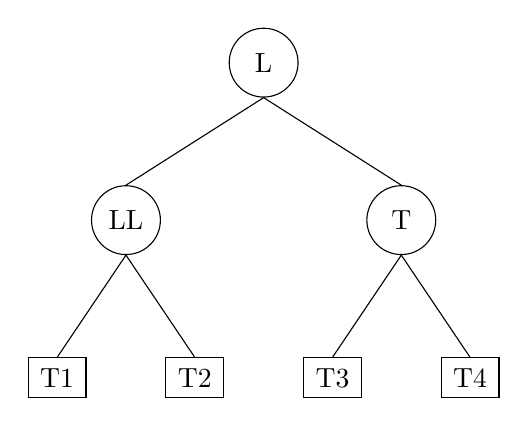
\begin{tikzpicture}

        \Tree [.\node[node_a]{L};
        [.\node[node_a]{LL};
        [.\node[subtree]{T1}; ]
        [.\node[subtree]{T2}; ]
        ]
        [.\node[node_a]{T};
        [.\node[subtree]{T3}; ]
        [.\node[subtree]{T4}; ]
        ]
        ]

\end{tikzpicture}
\end{document}
